% ---------------------------------------------------------------------------
% IEEE build.  Same sections, tables, figures and numbers as main.tex.
% Change one word on the \documentclass line to pick the route:
%   [journal]    IEEE Access / Transactions submission.  No page limit, so the
%                appendix binds into the paper and the author block becomes a
%                journal byline.  This is the default.
%   [conference] IEEE conference proceedings.  Two-column byline, and the
%                appendix ships separately as supplement_ieee.tex because
%                conference tracks cap at 8-10 pages.
% Compile: pdflatex main_ieee -> bibtex main_ieee -> pdflatex x2
% ---------------------------------------------------------------------------
\documentclass[journal]{IEEEtran}

% --- submission switches ---------------------------------------------------
% Double-blind review copy: hides the author block.
\newif\ifanon            \anonfalse
% Bind the appendix into the paper instead of shipping it as the supplement.
% Defaults to on for journals and off for conferences, where it would eat into
% the page limit; override either way by setting it after this line.
\newif\ifwithappendix
\ifCLASSOPTIONconference \withappendixfalse \else \withappendixtrue \fi
% Camera-ready copyright footer.  The venue issues the string; paste it into
% \pubidstring and flip this to \pubidtrue.
\newif\ifpubid           \pubidfalse
\newcommand{\pubidstring}{%
  979-8-XXXX-XXXX-X/26/\$31.00~\copyright~2026 IEEE}

% ---------------------------------------------------------------------------
% IEEEtran preamble.  Loaded only by main_ieee.tex; the preprint build
% (main.tex) keeps preamble.tex.  Two jobs: mirror preamble.tex, and make the
% shared section sources survive a two-column layout unedited.
% ---------------------------------------------------------------------------
\usepackage[T1]{fontenc}
\usepackage[utf8]{inputenc}
% No lmodern and no geometry: IEEEtran sets its own Times-like fonts and the
% margins the IEEE templates require.
\usepackage{amsmath,amssymb,amsthm}
\usepackage{graphicx}
\usepackage{booktabs}
\usepackage{caption}
\usepackage{subcaption}
\usepackage{microtype}
\usepackage{xcolor}
\usepackage{url}
\usepackage[numbers,sort&compress]{natbib}   % numeric [1], [2]-[4]; keeps \citet/\citep
\usepackage{enumitem}
\usepackage{stfloats}                        % lets wide floats sit at column bottoms
\usepackage[hidelinks,breaklinks]{hyperref}  % IEEEtran wants hyperref loaded last

\captionsetup{font=footnotesize,labelfont=bf,labelsep=period,skip=4pt}
\captionsetup[sub]{font=footnotesize,labelfont=bf}
\setlength{\parskip}{0pt}

\theoremstyle{definition}
\newtheorem{definition}{Definition}
\theoremstyle{plain}
\newtheorem{proposition}{Proposition}
\newtheorem{remark}{Remark}

\newcommand{\pone}{p_1}
\newcommand{\cov}{C}
\newcommand{\gap}{G}
\newcommand{\plur}{A}
\newcommand{\eff}{\eta}
\newcommand{\lift}{\Lambda}

% Display equations too wide for a 3.5in column are wrapped in \autofit by the
% section sources; in the one-column build it is the identity.
\newcommand{\autofit}[1]{%
  \resizebox{\columnwidth}{!}{$\displaystyle #1$}}

% --- Two-column float handling --------------------------------------------
% Every figure and table in this paper is designed full-width (7-8 column
% tables, wide multi-panel figures), so promote all of them to double-column
% floats rather than forking the section sources.  Inside a starred float
% \textwidth is the full page width, so the existing width=\textwidth graphics
% are already correct.
\makeatletter
\renewenvironment{figure}[1][\fps@figure]{\@dblfloat{figure}[#1]}{\end@dblfloat}
\renewenvironment{table}[1][\fps@table]{\@dblfloat{table}[#1]\footnotesize}{\end@dblfloat}
\makeatother

% Ten double-column floats in an eight-page paper: give LaTeX room so they do
% not all migrate to the end.
\renewcommand{\dbltopfraction}{0.9}
\renewcommand{\dblfloatpagefraction}{0.7}
\renewcommand{\textfraction}{0.07}
\setcounter{dbltopnumber}{4}
\setcounter{totalnumber}{6}

% Shared by main.tex, main_ieee.tex and supplement_ieee.tex.
\newcommand{\papertitle}{The Generator--Verifier Gap Predicts When
Multi-Agent LLM Architectures Beat a Compute-Matched Single Agent}

% Auto-generated by gvgap/report.py -- do not edit.
\newcommand{\nFamilies}{\textbf{??}}
\newcommand{\nPerFamily}{\textbf{??}}
\newcommand{\nTasks}{\textbf{??}}
\newcommand{\nModels}{\textbf{??}}
\newcommand{\nArch}{\textbf{??}}
\newcommand{\nCalib}{\textbf{??}}
\newcommand{\nTest}{\textbf{??}}
\newcommand{\nGenerations}{\textbf{??}}
\newcommand{\nFlip}{\textbf{??}}
\newcommand{\nCellsPositiveNaive}{\textbf{??}}
\newcommand{\nCellsFlipped}{\textbf{??}}
\newcommand{\medianNaiveLift}{\textbf{??}}
\newcommand{\medianMatchedLift}{\textbf{??}}
\newcommand{\fracMatchedNegative}{\textbf{??}}
\newcommand{\rTwoApriori}{\textbf{??}}
\newcommand{\rTwoTransfer}{\textbf{??}}
\newcommand{\maeApriori}{\textbf{??}}
\newcommand{\corrApriori}{\textbf{??}}
\newcommand{\nPredCells}{\textbf{??}}
\newcommand{\decisionAgreement}{\textbf{??}}
\newcommand{\nDecisionCells}{\textbf{??}}
\newcommand{\decisionBaseline}{\textbf{??}}
\newcommand{\decisionPrecision}{\textbf{??}}
\newcommand{\decisionRecall}{\textbf{??}}
\newcommand{\decisionLift}{\textbf{??}}
\newcommand{\etaProgSigMedian}{\textbf{??}}
\newcommand{\nSigCells}{\textbf{??}}
\newcommand{\nSigProgPositive}{\textbf{??}}
\newcommand{\rTwoJudgeArm}{\textbf{??}}
\newcommand{\nJudgeArmCells}{\textbf{??}}
\newcommand{\etaProgMedian}{\textbf{??}}
\newcommand{\etaJudgeMedian}{\textbf{??}}
\newcommand{\etaVoteMedian}{\textbf{??}}
\newcommand{\etaJudgeMin}{\textbf{??}}
\newcommand{\nEtaNegative}{\textbf{??}}
\newcommand{\nEtaCells}{\textbf{??}}
\newcommand{\Gmin}{\textbf{??}}
\newcommand{\Gmax}{\textbf{??}}
\newcommand{\nGnegative}{\textbf{??}}
\newcommand{\maxPositionBias}{\textbf{??}}
\newcommand{\minOrderConsistency}{\textbf{??}}
\newcommand{\minPairs}{\textbf{??}}
\newcommand{\nDroppedLowPairs}{\textbf{??}}
\newcommand{\rTwoAprioriNoFilter}{\textbf{??}}
\newcommand{\nCitTopics}{\textbf{??}}
\newcommand{\citHallucRate}{\textbf{??}}
\newcommand{\citPone}{\textbf{??}}
\newcommand{\citCoverage}{\textbf{??}}
\newcommand{\citEtaLLM}{\textbf{??}}
\newcommand{\citEtaAPI}{\textbf{??}}
\newcommand{\citG}{\textbf{??}}
\newcommand{\citPredEta}{\textbf{??}}
\newcommand{\citSaysReal}{\textbf{??}}
\newcommand{\citLLMTokens}{\textbf{??}}
\newcommand{\citAccLLM}{\textbf{??}}
\newcommand{\citAccAPI}{\textbf{??}}
\newcommand{\nCitUnresolved}{\textbf{??}}
\newcommand{\citUnparsed}{\textbf{??}}
\newcommand{\citParseable}{\textbf{??}}
\newcommand{\citHallucLoose}{\textbf{??}}
\newcommand{\citHallucMid}{\textbf{??}}
\newcommand{\citTPR}{\textbf{??}}
\newcommand{\citTNR}{\textbf{??}}
\newcommand{\citMedianRatio}{\textbf{??}}
\renewcommand{\nFamilies}{6}
\renewcommand{\nPerFamily}{90}
\renewcommand{\nTasks}{540}
\renewcommand{\nModels}{2}
\renewcommand{\nArch}{8}
\renewcommand{\nCalib}{30}
\renewcommand{\nTest}{60}
\renewcommand{\nGenerations}{21,847}
\renewcommand{\nFlip}{47\%}
\renewcommand{\nCellsPositiveNaive}{49}
\renewcommand{\nCellsFlipped}{23}
\renewcommand{\medianNaiveLift}{+0.036}
\renewcommand{\medianMatchedLift}{-0.028}
\renewcommand{\fracMatchedNegative}{56\%}
\renewcommand{\rTwoApriori}{0.84}
\renewcommand{\rTwoTransfer}{0.80}
\renewcommand{\maeApriori}{0.036}
\renewcommand{\corrApriori}{0.92}
\renewcommand{\nPredCells}{24}
\renewcommand{\decisionAgreement}{73\%}
\renewcommand{\nDecisionCells}{26}
\renewcommand{\decisionBaseline}{61.5\%}
\renewcommand{\decisionLift}{11.5}
\renewcommand{\decisionPrecision}{0.64}
\renewcommand{\decisionRecall}{0.70}
\renewcommand{\minPairs}{10}
\renewcommand{\nDroppedLowPairs}{2}
\renewcommand{\rTwoAprioriNoFilter}{0.85}
\renewcommand{\nSigCells}{22}
\renewcommand{\nSigProgPositive}{7}
\renewcommand{\etaProgSigMedian}{+0.183}
\renewcommand{\rTwoJudgeArm}{0.52}
\renewcommand{\nJudgeArmCells}{10}
\renewcommand{\etaProgMedian}{1.00}
\renewcommand{\etaJudgeMedian}{0.01}
\renewcommand{\etaVoteMedian}{0.19}
\renewcommand{\etaJudgeMin}{-0.39}
\renewcommand{\nEtaNegative}{5}
\renewcommand{\nEtaCells}{38}
\renewcommand{\Gmin}{-0.27}
\renewcommand{\Gmax}{+0.42}
\renewcommand{\nGnegative}{1}
\renewcommand{\minOrderConsistency}{0.00}
\renewcommand{\maxPositionBias}{1.00}
\renewcommand{\nCitTopics}{40}
\renewcommand{\nCitUnresolved}{0}
\renewcommand{\citHallucRate}{97.2\%}
\renewcommand{\citPone}{0.03}
\renewcommand{\citCoverage}{0.15}
\renewcommand{\citEtaLLM}{0.00}
\renewcommand{\citEtaAPI}{1.00}
\renewcommand{\citG}{-0.67}
\renewcommand{\citPredEta}{-0.18}
\renewcommand{\citSaysReal}{15\%}
\renewcommand{\citLLMTokens}{32,206}
\renewcommand{\citAccLLM}{0.03}
\renewcommand{\citAccAPI}{0.15}
\renewcommand{\citUnparsed}{36}
\renewcommand{\citParseable}{284}
\renewcommand{\citMedianRatio}{0.63}
\renewcommand{\citHallucMid}{87\%}
\renewcommand{\citHallucLoose}{69\%}
\renewcommand{\citTPR}{0.25}
\renewcommand{\citTNR}{0.85}


\ifpubid
  \IEEEoverridecommandlockouts
  \IEEEpubid{\makebox[\columnwidth]{\pubidstring\hfill}%
    \hspace{\columnsep}\makebox[\columnwidth]{}}
\fi

\begin{document}

\title{\papertitle}

\ifanon
  \ifCLASSOPTIONconference
    \author{\IEEEauthorblockN{Anonymous Submission}
    \IEEEauthorblockA{Paper ID \#XXXX}}
  \else
    \author{Anonymous Submission}
  \fi
\else
  \ifCLASSOPTIONconference
    \author{%
    \IEEEauthorblockN{Madhavam Pratap Shahi}
    \IEEEauthorblockA{Independent Researcher\\
    madhavam.shahi.12@gmail.com}
    \and
    \IEEEauthorblockN{Kavish Soningra}
    \IEEEauthorblockA{Independent Researcher}
    \and
    \IEEEauthorblockN{Nagendra Chaudhary}
    \IEEEauthorblockA{Independent Researcher}
    }
  \else
    \author{Madhavam Pratap Shahi, Kavish Soningra, and Nagendra Chaudhary%
    \thanks{The authors are independent researchers. Correspondence:
    madhavam.shahi.12@gmail.com. Code, data and every cached generation:
    \url{https://github.com/madhavamshahi/generator-verifier-gap}.}}
    \markboth{Preprint submitted to IEEE}{Shahi \MakeLowercase{\textit{et al.}}:
    The Generator--Verifier Gap}
  \fi
\fi

\maketitle

\begin{abstract}
% Shared by main.tex (article) and main_ieee.tex (IEEEtran).
Multi-agent architectures built from large language models are widely deployed,
but reports of their benefit conflict, and practitioners have no way to
anticipate whether one will help before building it. We argue two fixable
problems explain the disagreement: baselines are rarely matched on compute, and
no measurable task property has been identified that governs the outcome. We
show that a $k$-agent ensemble's accuracy decomposes exactly into
\emph{coverage}---the chance any of its candidates is correct---and
\emph{selection efficiency}, the fraction of that headroom its selector
converts. We then give a latent-score model that turns a cheap pairwise probe,
the \textbf{generator--verifier gap} $\gap$, into a parameter-free prediction of
selection efficiency. Across \nTasks{} tasks in \nFamilies{} families spanning
the verification spectrum, \nModels{} model scales and \nArch{} architectures,
with exact token accounting over \nGenerations{} generations, we find that
against a single agent priced at the same token budget, \nFlip{} of the apparent
multi-agent gains disappear and \fracMatchedNegative{} of all configurations are
net negative. Diagnostics measured on \nCalib{} calibration tasks predict held-out lift with
$R^2=\rTwoApriori{}$ (Pearson $r=\corrApriori{}$), with no fitted parameters and
without the multi-agent system ever being constructed. A case study on citation generation shows the same split in a deployed setting:
an external registry check attains selection efficiency $\citEtaAPI{}$ at zero
token cost, while the same model used as its own critic attains
$\citEtaLLM{}$. The pattern that survives is narrow: ensembles selected by an external program
verifier gain reliably, self-consistency gains where the answer distribution is
peaked on the truth, and ensembles selected by the model judging itself gain
nowhere. Multi-agent structure is not a general accuracy technique; it is a way
of spending compute that pays off exactly when checking an answer is easier
than producing one.

\end{abstract}

\begin{IEEEkeywords}
large language models, multi-agent systems, test-time compute, verification,
ensemble selection, benchmarking
\end{IEEEkeywords}

% Lengthens the first column that the copyright footer would otherwise shorten.
\ifpubid\IEEEpubidadjcol\fi

\section{Introduction}

Multi-agent architectures built from large language models are now routine
engineering practice. Frameworks such as AutoGen, MetaGPT and ChatDev
\citep{wu2023autogen,hong2024metagpt,qian2024chatdev} let a practitioner
decompose a task across several model instances that propose, critique and
aggregate one another's work, and reported gains over a single model are
common. Yet the picture from the literature is contradictory. Multi-agent
debate improves factuality and reasoning on some benchmarks
\citep{du2023debate}; simply sampling more answers and voting captures much of
the same benefit \citep{wang2023selfconsistency,li2024moreagents}; and a recent
study of deployed multi-agent systems finds failure rates high enough to
question whether the additional structure is doing useful work at all
\citep{cemri2025why}. Practitioners deciding whether to build a multi-agent
system therefore have no principled way to anticipate the answer, and the
prevailing method---build it, then measure---is expensive and often
inconclusive.

We argue that two problems explain most of this disagreement, and that both
are fixable.

\textbf{The baseline is usually not compute-matched.} A system of $k$ agents
spends roughly $k$ times the tokens of a single agent. Comparing it against one
agent that produced one answer credits the architecture for compute that any
method could have spent. The honest comparison prices the single agent at the
same budget---letting it think longer, or revise its own answer---and asks
whether \emph{coordination}, rather than \emph{compute}, produced the gain.
This concern has been raised for agent evaluation generally
\citep{kapoor2024agents} and for repeated sampling in particular
\citep{brown2024monkeys,snell2024scaling,stroebl2024limits}, but
compute-matched comparison is still not standard practice in the multi-agent
literature.

\textbf{There is no measurable quantity that says when to expect a gain.}
Existing accounts are largely taxonomic: they describe what multi-agent systems
do, or catalogue how they fail, without predicting where gains will appear.
What is missing is a property of the \emph{task and model together} that can be
measured cheaply, in advance, and that determines the answer.

This paper supplies that quantity. Our starting point is an observation that is
almost trivial once stated but that organises the entire empirical picture: an
ensemble of $k$ agents can only ever be as good as the best candidate it
produces, and it realises that potential only to the extent that its selection
mechanism can tell good candidates from bad. Writing $\pone$ for single-sample
accuracy, $\cov(k)$ for the probability that at least one of $k$ samples is
correct, and $A_\sigma(k)$ for the accuracy of a system using selector $\sigma$,
\begin{equation}
A_\sigma(k) \;=\; \pone + \eff_\sigma(k)\,\bigl(\cov(k) - \pone\bigr),
\label{eq:decomp-intro}
\end{equation}
where $\eff_\sigma(k) \in [0,1]$ is the fraction of the available
\emph{coverage headroom} $\cov(k)-\pone$ that the selector converts into
accuracy. Multi-agent gains require both factors to be non-trivial: headroom
without a discriminating selector is wasted, and a perfect selector on a pool
with no headroom has nothing to find.

The useful consequence is that both factors can be estimated \emph{before}
building the system, from a small labelled calibration set. Coverage headroom
needs only repeated sampling. For selection we introduce the
\textbf{generator--verifier gap} $\gap$: the probability, in excess of chance,
that the model prefers a correct candidate over an incorrect one when shown
both. Because $\gap$ is a \emph{pairwise} quantity while selection is
\emph{listwise}, we supply the link with a latent-score model
(Section~\ref{sec:framework}) that turns a measured $\gap$ into a
parameter-free prediction of $\eff$. Verifier-free aggregation such as
self-consistency needs no verifier at all and is governed by a second
diagnostic, \textbf{plurality alignment} $\plur$, which measures how well the
modal answer tracks the truth.

We test this on \nTasks{} tasks spanning six families chosen to span the
verification spectrum---from constraint-satisfaction problems whose answers can
be checked in a line of code, to transitive-ordering puzzles where confirming
an answer means redoing the derivation---across \nModels{} model scales and
\nArch{} architectures, all with exact token accounting. Our contributions:

\begin{enumerate}[leftmargin=1.4em,itemsep=2pt,topsep=3pt]
\item \textbf{A decomposition and a theory.} Equation~\eqref{eq:decomp-intro}
  separates a multi-agent system's accuracy into coverage and selection
  efficiency, and a latent-score model predicts selection efficiency from the
  pairwise gap $\gap$ with no free parameters (Section~\ref{sec:framework}).
\item \textbf{Token-matched evidence that most multi-agent gains are compute, not
  coordination.} Against a single agent priced at the same token budget,
  \nFlip{} of the architecture--task cells that appear to gain lose that gain,
  and the median configuration moves from \medianNaiveLift{} to
  \medianMatchedLift{}---a change of sign (Section~\ref{sec:results}).
\item \textbf{A prospective diagnostic.} Measured on \nCalib{} calibration
  tasks and passed through the model with no fitted parameters, the
  diagnostics predict held-out lift with $R^2 = \rTwoApriori{}$ without the
  multi-agent system ever being built. As a binary build/don't-build rule they
  are weaker---\decisionAgreement{} correct against a \decisionBaseline{}
  majority baseline---and we report that gap rather than the raw accuracy.
\item \textbf{A case study in a deployed setting.} On citation generation,
  where fabricated output is a known failure mode, an external registry check
  converts nearly all available headroom at zero token cost while the same
  model used as its own critic performs near chance
  (Section~\ref{sec:casestudy}).
\end{enumerate}

Our headline practical finding is a negative result with a constructive
remedy. Multi-agent structure is not a general-purpose accuracy technique; it
is a way of spending compute that pays off precisely when an asymmetry exists
between producing an answer and checking one. Where that asymmetry is absent,
the same tokens are better spent on a single agent---and where it is present,
the effective move is usually not another language-model critic but an external
check, which in our experiments costs no tokens at all.

\section{Related Work}
\label{sec:related}

\paragraph{Repeated sampling and test-time compute.}
Drawing many samples and keeping the best is the oldest form of test-time
scaling. \citet{chen2021codex} introduced the unbiased $\mathrm{pass}@k$
estimator we use for coverage; \citet{brown2024monkeys} showed coverage
continues to grow over orders of magnitude of samples, and
\citet{snell2024scaling} studied how best to allocate a fixed test-time budget.
This line establishes that the \emph{coverage} factor in
Equation~\eqref{eq:decomp-intro} is typically large. It also makes clear that
coverage alone is not accuracy: converting it requires a selector, and
\citet{stroebl2024limits} show formally that an imperfect verifier caps the
returns from resampling. Our contribution relative to that work is to make the
selector's contribution a \emph{measurable, predictable} quantity, tied to a
diagnostic that can be run before the system exists, and to evaluate it against
a compute-matched single agent rather than against a single sample.

\paragraph{Aggregation without a verifier.}
Self-consistency \citep{wang2023selfconsistency} takes a majority vote over
sampled reasoning chains and needs no verifier whatsoever. \citet{li2024moreagents}
find that this simple sampling-and-voting procedure scales with the number of
agents and often matches more elaborate multi-agent designs. Our plurality
alignment diagnostic is the property these methods implicitly rely on: that the
sampling distribution is peaked on the correct answer. We treat it as a second,
separate mechanism rather than folding it into verification, because our data
show families where voting helps while the model's verifier is at or below
chance.

\paragraph{Verifiers and judges.}
Training a separate verifier is highly effective when supervision is available
\citep{cobbe2021gsm8k,lightman2024verify,li2023stepaware}. In deployed
multi-agent systems the verifier is more often the same model prompted to
judge, a practice whose biases---including position bias---are documented by
\citet{zheng2023judge}. A related body of work finds that models are poor at
correcting their own reasoning without external signal
\citep{huang2024cannot,valmeekam2023selfcritique}, tempering the optimism of
self-refinement approaches \citep{madaan2023selfrefine}. The
generator--verifier gap makes this a quantity rather than a verdict: the same
model can be an excellent verifier on one family and a below-chance one on
another, and we measure which.

\paragraph{Multi-agent frameworks and their failures.}
Debate \citep{du2023debate} and role-structured frameworks
\citep{wu2023autogen,hong2024metagpt,qian2024chatdev} are the dominant designs.
\citet{cemri2025why} analyse why such systems fail and produce a taxonomy of
failure modes. Our account is complementary and predictive rather than
diagnostic: instead of classifying failures after the fact, we identify a
measurable precondition for success and show it forecasts the outcome.

\paragraph{Cost-aware evaluation.}
\citet{kapoor2024agents} argue that agent evaluations systematically neglect
cost, and that controlling for it changes conclusions. We adopt that stance for
multi-agent architecture specifically, reporting every result against a single
agent priced at the identical token budget, and we find the correction is not
cosmetic: it flips the sign of a substantial share of apparent gains.

\section{Framework}
\label{sec:framework}

\subsection{Setup}

Fix a task distribution $\mathcal{T}$ and a generator $\pi$ (a language model
with a decoding temperature). For a task $t$, drawing a sample $y \sim \pi(t)$
yields a correct answer with probability $\pone(t)$, and we write
$\pone = \mathbb{E}_t[\pone(t)]$ for the single-sample accuracy. A
\emph{$k$-agent ensemble} draws $y_1,\dots,y_k \sim \pi(t)$ independently and
applies a \emph{selector} $\sigma$ that returns one index. We write
$A_\sigma(k)$ for the resulting accuracy.

Two reference selectors bound the rest. The \emph{oracle} selector returns a
correct candidate whenever one exists, so its accuracy is the coverage
\begin{equation}
\cov(k) \;=\; \mathbb{E}_t\bigl[\Pr(\exists\, i \le k : y_i \text{ correct})\bigr],
\end{equation}
which we estimate with the unbiased $\mathrm{pass}@k$ estimator of
\citet{chen2021codex} from a pool of $n \ge k$ samples. The
\emph{uninformative} selector chooses an index independently of correctness;
its accuracy is $\pone$ for every $k$, since each candidate is marginally
correct with probability $\pone$.

\subsection{The coverage--selection decomposition}

\begin{definition}[Selection efficiency]
For a selector $\sigma$ with $\cov(k) \neq \pone$,
\begin{equation}
\eff_\sigma(k) \;=\; \frac{A_\sigma(k) - \pone}{\cov(k) - \pone}.
\label{eq:eta}
\end{equation}
\end{definition}

\begin{proposition}[Decomposition]
\label{prop:decomp}
For any selector, $A_\sigma(k) = \pone + \eff_\sigma(k)(\cov(k)-\pone)$.
An uninformative selector has $\eff_\sigma(k)=0$ and the oracle has
$\eff_\sigma(k)=1$. Every selector satisfies $\eff_\sigma(k) \le 1$;
$\eff_\sigma(k) < 0$ is attainable and indicates a selector anti-correlated
with correctness.
\end{proposition}

\begin{proof}
The identity is Equation~\eqref{eq:eta} rearranged. For the uninformative
selector, selection is independent of correctness, so the chosen candidate is
correct with its marginal probability $\pone$, giving $\eff=0$. For the oracle
$A_\sigma(k)=\cov(k)$ gives $\eff=1$. No selector can exceed $\cov(k)$, since it
returns one of the generated candidates and is correct only if that candidate
is; hence $\eff_\sigma(k)\le 1$. Nothing prevents $A_\sigma(k) < \pone$---a
selector that systematically prefers confident errors---so $\eff_\sigma(k)$ is
not bounded below by zero.
\end{proof}

Proposition~\ref{prop:decomp} is elementary, and deliberately so: its value is
that it names the two factors that any multi-agent gain must pass through, and
both are separately measurable. It also makes the failure modes explicit.
A selector cannot rescue a pool with no headroom ($\cov(k) \approx \pone$), and
headroom is worthless without a selector that can find it ($\eff \approx 0$).
The possibility $\eff < 0$ is not hypothetical; we observe it
(Section~\ref{sec:results}).

\subsection{From pairwise discrimination to listwise selection}

The decomposition is useless prospectively unless $\eff$ can be estimated
without building the system. We estimate it from a cheaper probe.

\begin{definition}[Generator--verifier gap]
Present the model with a task and two candidate answers, one correct and one
incorrect, in randomised order, and ask which is correct. Let $q$ be the
probability it answers correctly. The generator--verifier gap is
$\gap = 2q - 1 \in [-1, 1]$.
\end{definition}

$\gap=0$ means the model cannot distinguish its own correct answers from its
incorrect ones; $\gap=1$ means it always can; $\gap<0$ means it is
systematically misled. Crucially $\gap$ is a \emph{pairwise} quantity, while a
$k$-agent ensemble makes a \emph{listwise} choice. We bridge the two with a
minimal latent-score model.

\begin{definition}[Latent-score selector]
\label{def:latent}
The verifier assigns candidate $i$ a score $s_i$, drawn independently from
$\mathcal{N}(\delta,1)$ if $y_i$ is correct and $\mathcal{N}(0,1)$ otherwise,
and selects $\arg\max_i s_i$.
\end{definition}

\begin{proposition}[Identification and prediction]
\label{prop:latent}
Under Definition~\ref{def:latent}, the pairwise preference probability is
$q = \Phi(\delta/\sqrt{2})$, so an observed gap identifies the separation
\begin{equation}
\delta = \sqrt{2}\,\Phi^{-1}\!\left(\tfrac{1+\gap}{2}\right)
\label{eq:delta}
\end{equation}
with no free parameters. If $c$ of the $k$ candidates are correct, the
probability of selecting a correct one is
\begin{equation}
P(c,k,\delta) \;=\; \Pr\Bigl(\max_{j\le c} X_j > \max_{j \le k-c} Z_j\Bigr),
\quad X_j \sim \mathcal{N}(\delta,1),\; Z_j \sim \mathcal{N}(0,1),
\label{eq:listwise}
\end{equation}
and the predicted selector accuracy is
$\hat{A}_\sigma(k) = \mathbb{E}_{c}\bigl[P(c,k,\delta)\bigr]$, with the
expectation taken over the observed distribution of $c$. The predicted
selection efficiency follows from Equation~\eqref{eq:eta}.
\end{proposition}

\begin{proof}
$s_{\text{correct}} - s_{\text{incorrect}} \sim \mathcal{N}(\delta, 2)$, so
$q = \Pr(s_{\text{correct}} > s_{\text{incorrect}}) = \Phi(\delta/\sqrt{2})$,
which inverts to Equation~\eqref{eq:delta} since $\Phi$ is strictly increasing.
Equation~\eqref{eq:listwise} is the definition of the argmax event conditional
on $c$; $P(0,k,\delta)=0$ and $P(k,k,\delta)=1$. Averaging over $c$ gives
$\hat{A}_\sigma(k)$.
\end{proof}

Two things make Proposition~\ref{prop:latent} usable. First, $\gap$ and the
distribution of $c$ are both estimable from a small labelled calibration set by
sampling $k$ answers per task---no multi-agent system need be built. Second,
nothing is fitted: Equation~\eqref{eq:delta} pins $\delta$, and
Equation~\eqref{eq:listwise} is evaluated by simulation. The model is
intentionally the simplest that respects the pairwise/listwise distinction; it
assumes scores are conditionally independent and equally dispersed, and
Section~\ref{sec:results} reports where those assumptions hold and where they
fail.

\subsection{Aggregation without a verifier}

Self-consistency uses no verifier, so $\gap$ cannot explain it. It relies
instead on the sampling distribution concentrating on the truth.

\begin{definition}[Plurality alignment]
Let $\hat{y}$ be the modal answer among $k$ samples. Plurality alignment is
$\plur = \Pr(\hat{y} \text{ correct}) - \pone$, the accuracy advantage of the
mode over a single sample.
\end{definition}

$\plur$ is also estimable from the same calibration pool at no extra cost, and
it is the natural predictor of self-consistency's lift. Separating $\gap$ from
$\plur$ matters empirically: we find families where $\plur > 0$ while $\gap
\le 0$, so a system can benefit from voting while the very same model is
useless as a judge.

\subsection{Token-matched lift and the decision rule}
\label{sec:matched}

Let $\mathcal{C}(\cdot)$ denote total tokens consumed per task, prompt plus
completion. A $k$-agent ensemble costs roughly $k$ times a single sample. We
therefore compare it not against one sample but against the \emph{single-agent
frontier} $a(\cdot)$: the accuracy a single agent reaches when given the same
budget to spend serially, by generating and then revising its own answer.

\begin{definition}[Token-matched lift]
For an architecture $\mathcal{A}$ with cost $\mathcal{C}(\mathcal{A})$,
\begin{equation}
\lift(\mathcal{A}) \;=\; A(\mathcal{A}) \;-\; a\bigl(\mathcal{C}(\mathcal{A})\bigr).
\end{equation}
\end{definition}

$\lift > 0$ is the claim a multi-agent architecture must support: that spending
the budget across coordinating agents beats spending it inside one. Combining
with Proposition~\ref{prop:decomp} gives the rule we evaluate prospectively:

\begin{equation}
\textbf{build the ensemble} \iff
\underbrace{\hat{\eff}_\sigma(k)\bigl(\hat{\cov}(k) - \hat{\pone}\bigr)}_{\text{predicted from calibration}}
\;>\;
\underbrace{a\bigl(\mathcal{C}(\mathcal{A})\bigr) - \pone}_{\text{sequential gain}} .
\label{eq:rule}
\end{equation}

Every quantity on the left is measurable in advance from
Proposition~\ref{prop:latent} and repeated sampling; the right-hand side
requires only running one agent at a larger budget. Section~\ref{sec:results}
tests both the numerical prediction and the binary decision it implies.

\section{Experimental Setup}
\label{sec:setup}

\subsection{Task families}

We need tasks that span the verification spectrum, not a single benchmark. We
use six families, \nPerFamily{} tasks each (\nTasks{} total), chosen so that the
cost of \emph{checking} an answer varies by orders of magnitude while the cost
of \emph{producing} one does not.

\begin{description}[leftmargin=0pt,itemsep=2pt,topsep=3pt,font=\normalfont\itshape]
\item[CSP (synthetic).] ``Find the smallest integer $n>L$ leaving remainder
  $r_1$ mod $m_1$ and $r_2$ mod $m_2$.'' Checking is two modulo operations and
  an upward scan; producing requires the Chinese remainder theorem or a search.
  The high-asymmetry anchor.
\item[WordCon (synthetic).] ``Write one sentence about $X$, exactly $N$ words
  long, containing words $w_1$ and $w_2$.'' Checking is a token count and two
  substring tests. A high-asymmetry task in a natural-language rather than
  symbolic domain.
\item[MBPP \citep{austin2021mbpp}.] Python function synthesis with executable
  tests. The one family admitting a near-perfect external verifier, which lets
  us separate the ceiling imposed by coverage from the ceiling imposed by the
  selector.
\item[GSM8K \citep{cobbe2021gsm8k}.] Grade-school word problems with a numeric
  answer. Checking means redoing the arithmetic, but the answer is a short
  canonical string, so voting applies.
\item[ARC-Challenge \citep{clark2018arc}.] Multiple-choice science questions.
  Verification is essentially re-answering; the answer space is tiny.
\item[Logic (synthetic).] Transitive-ordering puzzles: a shuffled chain of
  pairwise comparisons over $4$--$6$ entities, asking for the extremum.
  Confirming a proposed answer means re-running the same derivation. The
  low-asymmetry anchor.
\end{description}

Three families are generated programmatically from a fixed seed. This is
deliberate: synthetic families carry no benchmark-contamination risk, their
difficulty is tunable, and their verifiers are exact rather than approximate.
Each family is split \nCalib{}/\nTest{} into a calibration and a held-out set
\emph{before any model is run}, since our central prediction claim requires
that the split not be chosen after seeing results.

\subsection{Models}

We use the Qwen2.5-Instruct family \citep{qwen2024qwen25} at 0.5B and 1.5B
parameters, in \texttt{bfloat16} without quantisation, run locally with MLX on
a single Apple M4 Pro. Using one family across scales isolates model size from
architecture and tokenizer differences, and running locally makes the entire
study reproducible at zero marginal cost---a deliberate choice given that our
claims concern compute accounting. The released code runs a third scale (3B)
unchanged; we report two because the full grid at three scales exceeds the
compute we allotted, and we prefer two scales at full statistical power to
three at half. Sampling uses temperature $0.7$ and
top-$p$ $0.95$; the judge and pairwise probes are run at temperature $0$.
Section~\ref{sec:limitations} discusses what this does and does not license us
to say about frontier-scale models.

\subsection{Architectures}

All selector-based architectures read the \emph{same} pool of $n=8$ independent
samples per task, so differences between them are attributable to selection
alone, with the generator held fixed and comparisons paired at the task level.

\begin{description}[leftmargin=0pt,itemsep=2pt,topsep=3pt,font=\normalfont\itshape]
\item[Single.] One sample. The $k=1$ reference point.
\item[Sequential refine.] One agent that generates, then revises its own answer
  for $r-1$ further rounds, $r \in \{1,2,3,4\}$. This is the compute-matched
  single-agent baseline and traces the frontier $a(\cdot)$.
\item[Self-consistency.] Majority vote over the canonical answers of $k$
  samples \citep{wang2023selfconsistency}. Undefined for families with no short
  canonical answer (WordCon, MBPP), which we report as such rather than forcing.
\item[Ensemble + LLM judge.] The same model, shown all $k$ candidates in
  randomised order, picks one.
\item[Ensemble + program verifier.] A non-LLM checker derived \emph{from the
  problem statement alone} selects the first passing candidate. Available for
  CSP, WordCon and MBPP. It consumes no model tokens.
\item[Ensemble + oracle.] Selects a correct candidate when one exists. Not
  deployable; reported as the coverage ceiling.
\item[Debate.] $3$ agents over $2$ or $3$ rounds, each round conditioned on the
  others' previous answers, with a final majority vote \citep{du2023debate}.
\end{description}

Selectors are evaluated at $k \in \{2,4,8\}$; for $k<8$ we average over three
random sub-pools to reduce variance.

\paragraph{Preventing verifier leakage.}
The program verifier must not see anything the generator did not. For CSP and
WordCon the constraints are fully stated in the prompt, so the checker is a
direct transcription of the problem. For MBPP the prompt shows one test case,
and the verifier may use \emph{only} that test; grading uses the held-out
remainder of the test list. Without this precaution the verifier would be
scored on the same signal used to select, inflating its apparent efficiency.

\subsection{Token accounting}

Every generation records its own prompt and completion token counts, and an
architecture's cost is the sum over all calls it makes, including judge and
debate turns. We count prompt tokens as well as completions because a judge
call that reads eight candidates is expensive even when its output is one word.
The program verifier's cost is recorded as zero model tokens; it runs in
milliseconds of CPU, which is the point of using it.

\subsection{Statistics}

All intervals are $95\%$ percentile bootstrap intervals over \emph{tasks}
($10{,}000$ resamples), since samples within a task are not independent.
Architecture comparisons are paired on the same task set. For token-matched
lift both arms are recomputed inside each bootstrap resample---the multi-agent
accuracy and the sequential frontier it is priced against---because the
baseline is itself an estimate; holding it fixed would understate the interval.
Where we report many comparisons at once, $p$-values are Holm--Bonferroni
adjusted. Coverage uses the unbiased $\mathrm{pass}@k$ estimator throughout.

\section{Results}
\label{sec:results}

We report five findings, in the order the framework implies: coverage exists
(R1), selectors mostly fail to convert it (R2--R3), compute-matching removes
most of what remains (R4), and the two cheap diagnostics predict all of this in
advance (R5).

\begin{figure}[t]
\centering
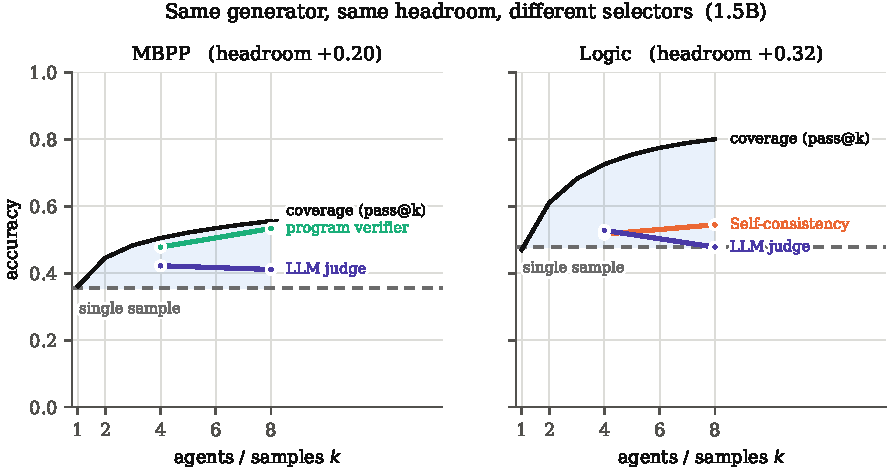
\includegraphics[width=\textwidth]{figures/fig1_thesis.pdf}
\caption{The decomposition on a high- and a low-asymmetry family. The shaded
band is coverage headroom---accuracy that already exists in the candidate
pool. Where a selector's curve sits inside that band is its selection
efficiency $\eff$. The two panels share a generator and differ only in how
checkable the task is.}
\label{fig:thesis}
\end{figure}

\subsection{R1: Coverage headroom is large and nearly universal}

\begin{figure}[t]
\centering
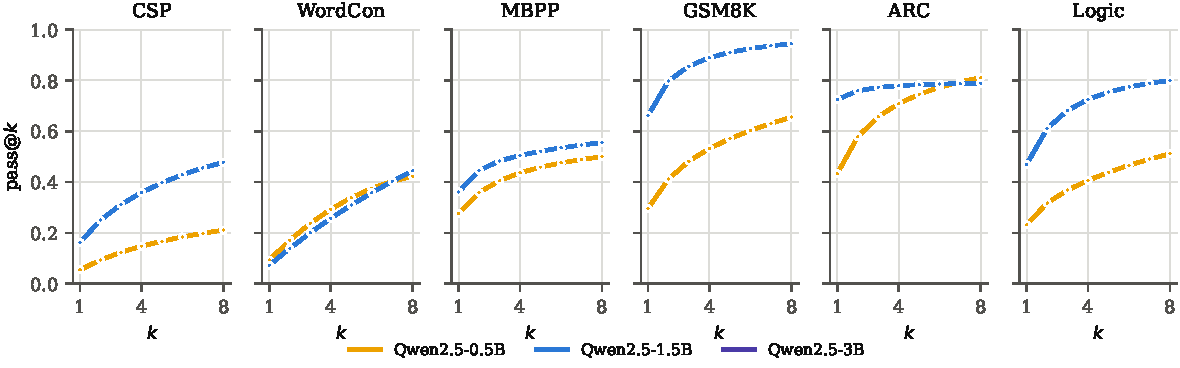
\includegraphics[width=\textwidth]{figures/fig2_coverage.pdf}
\caption{Unbiased $\mathrm{pass}@k$ by family and model. Headroom---the gap
between $k=1$ and $k=8$---is substantial almost everywhere, so the coverage
factor is rarely what limits a multi-agent system.}
\label{fig:coverage}
\end{figure}

Figure~\ref{fig:coverage} shows $\mathrm{pass}@k$ for every family and model.
Consistent with the repeated-sampling literature
\citep{brown2024monkeys,snell2024scaling}, coverage rises steeply with $k$:
sampling eight times rather than once adds substantial headroom in nearly every
cell. Table~\ref{tab:main} gives the corresponding single-sample accuracies.

The practical reading is that the first factor of
Equation~\eqref{eq:decomp-intro} is usually \emph{not} the binding constraint.
Multi-agent systems fail, when they fail, on the second factor.

\begin{table}[t]
\centering\small
\begin{tabular}{lrrrrrr}
\toprule
Architecture & CSP & WordCon & MBPP & GSM8K & ARC & Logic \\
\midrule
Single sample & 0.21 & 0.10 & 0.36 & 0.64 & 0.70 & 0.48 \\
Sequential refine & 0.34 & 0.03 & 0.39 & 0.67 & 0.64 & 0.40 \\
Self-consistency & 0.23 & -- & -- & 0.87 & 0.71 & 0.54 \\
Ensemble + LLM judge & 0.20 & 0.07 & 0.41 & 0.69 & 0.70 & 0.48 \\
Ensemble + program verifier & 0.48 & 0.44 & 0.53 & -- & -- & -- \\
Debate (3$\times$2) & 0.19 & 0.02 & 0.38 & 0.53 & 0.72 & 0.53 \\
\midrule
\textit{Ensemble + oracle} (ceiling) & 0.48 & 0.44 & 0.56 & 0.94 & 0.79 & 0.80 \\
\midrule
\multicolumn{7}{l}{\textit{mean tokens per task}} \\
\quad Single sample & 366 & 78 & 125 & 309 & 101 & 81 \\
\quad Sequential refine & 2,274 & 449 & 908 & 1,709 & 762 & 929 \\
\quad Ensemble + LLM judge & 5,012 & 849 & 1,454 & 4,052 & 1,028 & 961 \\
\quad Debate (3$\times$2) & 2,532 & 637 & 1,093 & 2,194 & 736 & 662 \\
\bottomrule
\end{tabular}
\caption{Accuracy by architecture and family, and mean token cost per task.
The oracle row is the coverage ceiling: it is not deployable, and the distance
between it and the deployable selectors is the accuracy the ensemble generated
but could not identify.}
\label{tab:main}
\end{table}

\subsection{R2: The generator--verifier gap varies enormously, and is sometimes negative}

\begin{table}[t]
\centering\small
\begin{tabular}{llrrrrrr}
\toprule
Model & Diagnostic & CSP & WordCon & MBPP & GSM8K & ARC & Logic \\
\midrule
Qwen2.5-0.5B & $\gap$ (verifier) & +0.00 & +0.00 & +0.00 & +0.00 & +0.00 & +0.00 \\
 & $\plur$ (plurality) & +0.03 & -- & -- & +0.13 & +0.03 & -0.07 \\
 & position bias & 1.00 & 0.00 & 0.20 & 1.00 & 1.00 & 1.00 \\
 & order consistency & 0.00 & 0.00 & 0.20 & 0.00 & 0.00 & 0.00 \\
\addlinespace
Qwen2.5-1.5B & $\gap$ (verifier) & +0.42 & -0.27 & +0.42 & +0.05 & +0.09 & +0.05 \\
 & $\plur$ (plurality) & +0.07 & -- & -- & +0.30 & +0.00 & +0.00 \\
 & position bias & 0.29 & 0.59 & 0.54 & 0.42 & 0.36 & 0.18 \\
 & order consistency & 0.58 & 0.45 & 0.58 & 0.65 & 0.00 & 0.16 \\
\addlinespace
\bottomrule
\end{tabular}
\caption{The two cheap diagnostics measured on the \nCalib{}-task calibration
split, with judge position bias (the rate at which the first-listed candidate
is chosen; $0.5$ is unbiased) and order consistency (how often the judge names
the same candidate when the two are presented in the opposite order; a judge
that simply picks a position scores $0$). $\gap$ ranges from \Gmin{} to \Gmax{};
\nGnegative{} cells are negative, meaning the model prefers its own incorrect
answers more often than its correct ones.}
\label{tab:diagnostics}
\end{table}

Table~\ref{tab:diagnostics} reports $\gap$ and $\plur$ per cell. The spread is
the central empirical fact of this paper: the same model, asked the same kind
of question---``which of these two answers is right?''---ranges from near-perfect
discrimination on families whose answers can be checked mechanically to
\emph{below chance} on families where checking means redoing the derivation.
\nGnegative{} of our cells have $\gap < 0$.

A negative gap deserves emphasis because it is not merely a small gain. It
means a model critic is an \emph{actively harmful} selector: it systematically
prefers wrong answers, so adding it to a pipeline reduces accuracy below
picking a candidate at random. Part of the mechanism is visible in the position
bias column, where the smallest model chooses the first-listed candidate up to
\maxPositionBias{} of the time, reproducing at small scale the bias documented
for stronger judges by \citet{zheng2023judge}. Order consistency falls as low
as \minOrderConsistency{}: on those cells the judge is not evaluating the
candidates at all, it is naming a position, and reversing the presentation
reverses its verdict.

Because a position-picking judge would otherwise inherit spurious
discrimination from any imbalance in which side happens to hold the correct
answer, every pair in our probe is presented twice, once in each order, and
$\gap$ averages over both. Under this counterbalancing a pure position-picker
scores exactly chance by construction. We flag this because our own first
implementation randomised the side independently per pair, which at
$n\approx20$ produced an apparent $\gap$ of $+0.40$ on a cell whose judge chose
the first option $100\%$ of the time.

\subsection{R3: Selection efficiency, not coverage, is what separates architectures}

\begin{figure}[t]
\centering
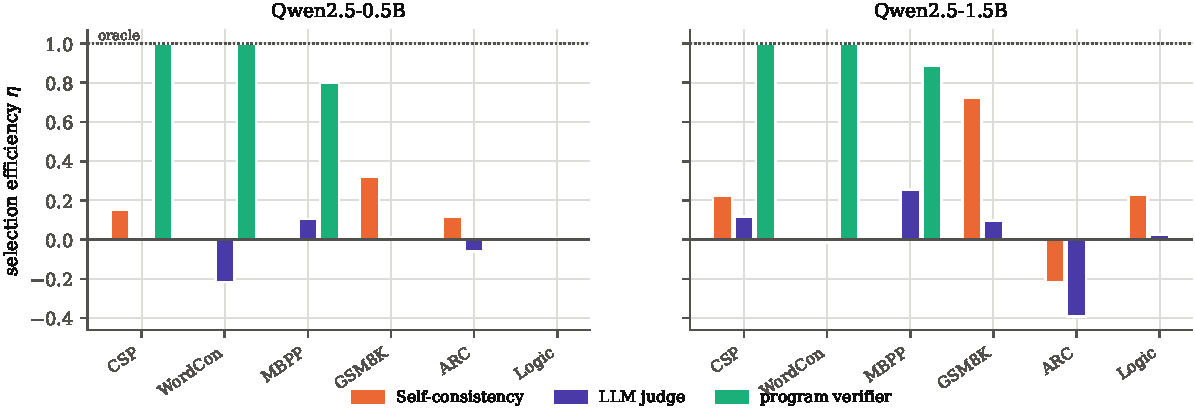
\includegraphics[width=\textwidth]{figures/fig3_eta.pdf}
\caption{Selection efficiency $\eff$ at $k=8$. A value of $1$ means the
selector captures all available headroom; $0$ means it does no better than
picking at random; negative means it does worse.}
\label{fig:eta}
\end{figure}

Figure~\ref{fig:eta} decomposes the architectures by $\eff$. Across
\nEtaCells{} measured cells the median program verifier attains
$\eff = \etaProgMedian{}$, the median self-consistency $\etaVoteMedian{}$, and
the median LLM judge $\etaJudgeMedian{}$, with a worst case of
$\etaJudgeMin{}$; \nEtaNegative{} cells are negative.

Two caveats keep this honest. First, for CSP and WordCon the program verifier
is a \emph{complete} checker---it tests exactly the property the grader
tests---so $\eff=1$ there is true by construction and demonstrates only that
the ceiling is attainable at zero token cost, not that verification is
magically easy. The informative case is MBPP, where the verifier sees one test
and grading uses held-out tests, so its efficiency is earned rather than
assumed. Second, self-consistency requires a canonical short answer and is
simply undefined for WordCon and MBPP; we report that rather than forcing a
degenerate clustering.

\subsection{R4: Token-matching removes most of the apparent benefit}

\begin{figure}[t]
\centering
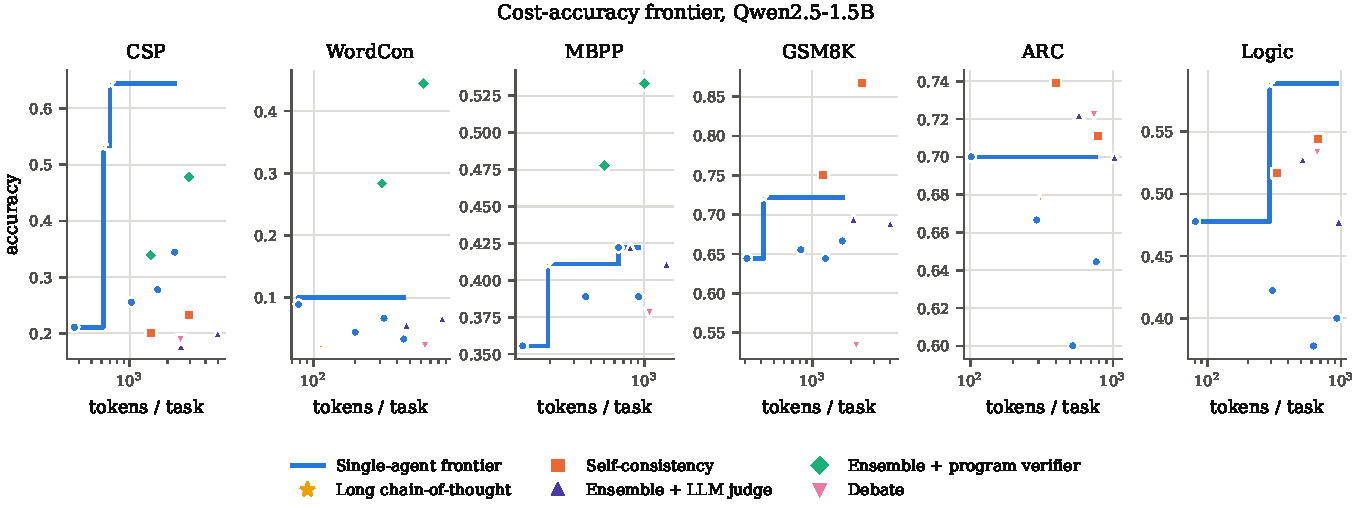
\includegraphics[width=\textwidth]{figures/fig4_frontier.pdf}
\caption{Accuracy against token cost. The line is the single-agent frontier:
the upper envelope of sequential refinement and long chain-of-thought at each
budget. A multi-agent point above the line earns its compute; a point below it
would have done better as one agent thinking longer.}
\label{fig:frontier}
\end{figure}

\begin{figure}[t]
\centering
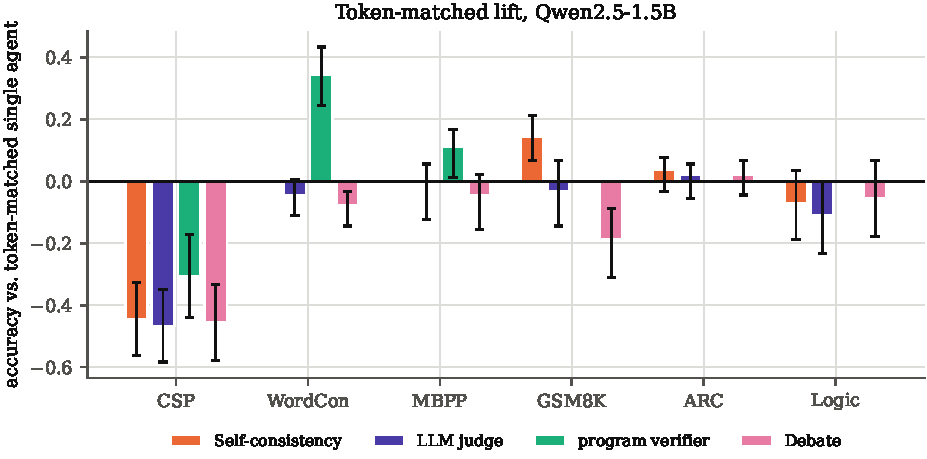
\includegraphics[width=0.82\textwidth]{figures/fig5_matched_lift.pdf}
\caption{Token-matched lift with $95\%$ cluster-bootstrap intervals, in which
both the multi-agent accuracy and the single-agent frontier are recomputed
inside every resample.}
\label{fig:matched}
\end{figure}

\begin{table}[t]
\centering\small
\begin{tabular}{lrrrr}
\toprule
Family & Self-consistency & LLM judge & program verifier & Debate (3$\times$2) \\
\midrule
CSP & $-0.444$$^{*}$ & $-0.467$$^{*}$ & $-0.306$$^{*}$ & $-0.456$$^{*}$ \\
WordCon & -- & $-0.044$ & $+0.344$$^{*}$ & $-0.078$ \\
MBPP & -- & $-0.011$ & $+0.111$$^{*}$ & $-0.044$ \\
GSM8K & $+0.144$$^{*}$ & $-0.033$ & -- & $-0.189$$^{*}$ \\
ARC & $+0.039$ & $+0.022$ & -- & $+0.022$ \\
Logic & $-0.072$ & $-0.111$ & -- & $-0.056$ \\
\bottomrule
\end{tabular}
\caption{Token-matched lift by family and architecture. $^{*}$ marks
Holm--Bonferroni adjusted $p<0.05$. Compare against the naive comparison
against a single sample, which is what most of the literature reports.}
\label{tab:matched}
\end{table}

This is the result with the most direct bearing on practice. Measured against a
single sample---the comparison most commonly reported---the median architecture
gains \medianNaiveLift{}. Measured against a single agent given the same token
budget, the median becomes \medianMatchedLift{}, and
\fracMatchedNegative{} of all configurations are net negative. Of the
\nCellsPositiveNaive{} cells that appear to benefit under the naive comparison,
\nCellsFlipped{} (\nFlip{}) do not survive compute-matching.

The architectures do not fail equally, and the pattern is the one the framework
predicts. Systems whose selector is an external program retain their advantage,
because their verification is both reliable and free. Systems whose selector is
the model judging itself lose most or all of theirs, because they pay $k$ times
the tokens for a selector whose $\gap$ does not support the choice. Debate is
the most expensive arm and among the weakest per token, which is consistent
with its gains being attributable to additional sampling rather than to the
exchange of arguments---the interpretation \citet{li2024moreagents} reach from
the opposite direction.

\subsection{R5: The diagnostics predict lift before the system is built}

\begin{figure}[t]
\centering
\begin{subfigure}{0.48\textwidth}
\centering
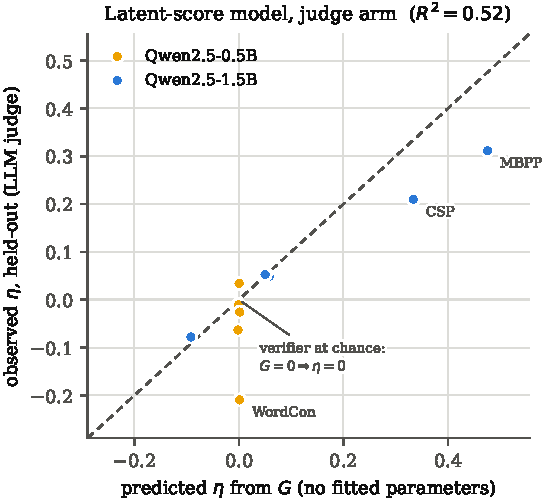
\includegraphics[width=\textwidth]{figures/fig8_theory.pdf}
\caption{Latent-score model: predicted versus observed $\eff$.}
\end{subfigure}\hfill
\begin{subfigure}{0.48\textwidth}
\centering
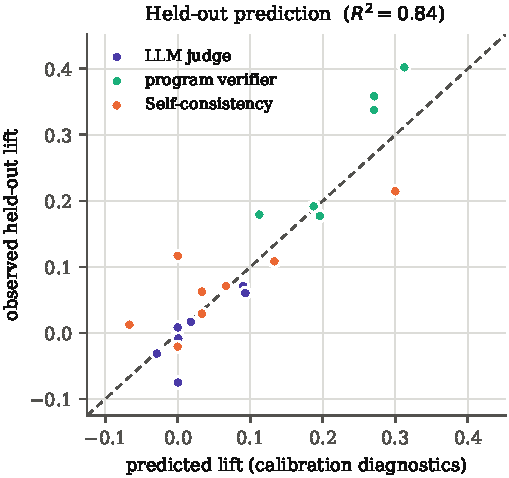
\includegraphics[width=\textwidth]{figures/fig6_prediction.pdf}
\caption{Held-out lift, predicted from calibration diagnostics.}
\end{subfigure}
\caption{Both panels compare against the identity line, not a fitted
regression: the theory predicts the \emph{value}, so a fitted slope would hide
bias.}
\label{fig:prediction}
\end{figure}

Finally we test whether the framework is usable prospectively. Features come
from the \nCalib{}-task calibration split only; targets come from the
\nTest{}-task held-out split; the split was fixed before any model ran.

A discriminating pair requires one correct and one incorrect candidate in the
same pool, so on families where accuracy is very low or very high, $\gap$ rests
on few comparisons. We therefore pre-specified a minimum of \minPairs{} scored
pairs for cells whose prediction depends on $\gap$, which excludes
\nDroppedLowPairs{} cells; without that filter the same analysis gives
$R^2 = \rTwoAprioriNoFilter{}$, so the conclusion does not rest on the choice.

Across \nPredCells{} cells, the a priori prediction---$\gap$ and $\plur$
measured on calibration, passed through Proposition~\ref{prop:latent}, with no
fitted parameters---attains $R^2 = \rTwoApriori{}$ against the identity line
(Pearson $r = \corrApriori{}$, mean absolute error \maeApriori{}). Simply transferring measured $\eff$ from calibration to held-out attains
$R^2 = \rTwoTransfer{}$, which upper-bounds what any diagnostic could achieve
given sampling noise; the a priori prediction essentially matches it, so the
cheap probe loses little against directly measuring the thing it estimates.

Restricted to the judge arm alone---where the latent-score model does all of
the work, rather than the coarse separation between verifier types---the
prediction attains $R^2 = \rTwoJudgeArm{}$ over \nJudgeArmCells{} cells
(Figure~\ref{fig:prediction}a). Two features of that panel are worth stating
plainly. Every cell with $\gap=0$ is predicted to have $\eff=0$ exactly, which
is not a fitted success but a property of the model; the observed values
scatter around zero as sampling noise. And at the high end the model
\emph{over}-predicts: the two cells with the largest gaps sit visibly below
the identity line. We take this as the expected cost of assuming
conditionally independent, equally dispersed scores---a listwise judge that
sees all candidates at once violates both---and we report it rather than
introducing a free parameter to absorb it.

Turned into the binary decision of Equation~\eqref{eq:rule}---build the ensemble,
or spend the tokens on one agent---the rule agrees with the token-matched
outcome in \decisionAgreement{} of \nDecisionCells{} cells, at precision
\decisionPrecision{} and recall \decisionRecall{}. We report that number
against the right yardstick rather than against chance: because multi-agent
architectures fail so often in our data, simply answering ``do not build'' every
time is already correct \decisionBaseline{} of the time, so the diagnostic buys
\decisionLift{} percentage points over that baseline. This is a real but modest
gain, and it is the weakest of our results. The continuous prediction is the
claim we would stand behind: the diagnostics estimate \emph{how much} an
architecture will gain far better than they resolve the knife-edge cases where
the gain is near zero, which is precisely where a binary rule is forced to
commit. A practitioner is better served by the predicted magnitude and its
uncertainty than by the rule's verdict.

That the majority baseline sits at \decisionBaseline{} is itself the finding
worth carrying away: across \nDecisionCells{} architecture--task pairs drawn
from the designs the literature recommends, the prior that multi-agent
structure will not survive compute-matching is correct more often than not.

\subsection{R6: How the diagnostics move with scale}

\begin{figure}[t]
\centering
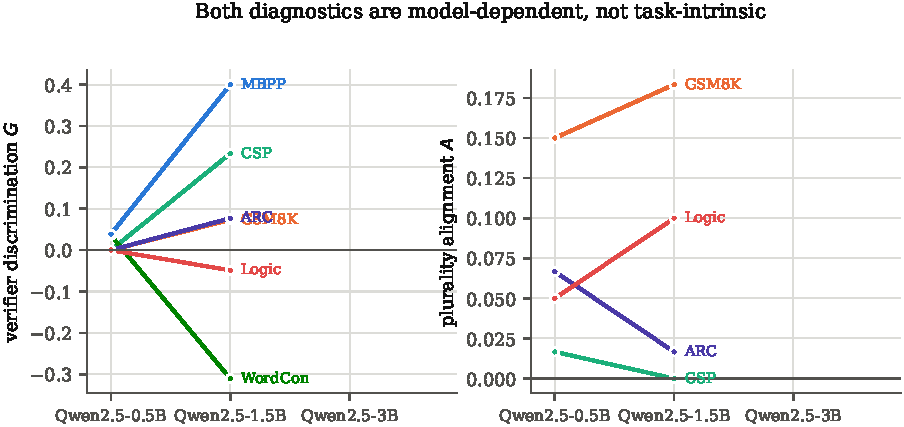
\includegraphics[width=0.85\textwidth]{figures/fig7_scale.pdf}
\caption{Both diagnostics across model scale. They are properties of a
(model, task) pair, not of the task alone, so they must be re-measured when
either changes.}
\label{fig:scale}
\end{figure}

Figure~\ref{fig:scale} contrasts $\gap$ and $\plur$ at 0.5B and 1.5B. The important
qualitative point is that neither is a property of the task alone: the same
family can move from a negative to a positive gap as the model grows, which
means a multi-agent design that fails at one scale may succeed at another and
vice versa. This is the mechanism we think underlies much of the disagreement in
the literature. We state explicitly what two points cannot do: they show the diagnostics are model-dependent, and they establish no trend and license no extrapolation. A third scale point is the single most valuable addition to this study, and the released code runs it unchanged.

\section{Case Study: Citation Verification}
\label{sec:casestudy}

The six families of Section~\ref{sec:setup} are controlled by construction. To
check that the framework says something useful about a task people actually
deploy language models on, we apply it to reference generation---a setting
where fabricated output is a known and consequential failure mode, and where an
external registry supplies a near-perfect verifier for the price of an HTTP
request.

The task ``produce a real published reference on topic $X$'' maps onto the
framework exactly. A generator proposes $k$ candidate references; a selector
picks one; ground truth is whether the reference exists. We ran this with
Qwen2.5-1.5B over \nCitTopics{} research topics spanning the sciences, drawing
$k=8$ candidate references per topic, and resolved every candidate against the
OpenAlex catalogue by fuzzy title match (threshold $0.88$), which supplies both
ground truth and one of the two selectors under comparison.

\paragraph{Resolution failures are not fabrications.}
A registry lookup can fail because the paper does not exist or because the
service is temporarily unavailable, and conflating the two would convert a
network condition into a measured hallucination. We retry with exponential
backoff and record any candidate we still cannot resolve as \emph{unresolved}
rather than absent; \nCitUnresolved{} candidates were excluded on this basis,
and a topic contributes to the analysis only if all eight of its candidates
resolved.

\subsection{Results}

The generator hallucinates heavily: \citHallucRate{} of proposed references
could not be found, so a single candidate is real with probability
$\citPone{}$. Coverage is much higher---at least one of eight candidates
resolves for $\citCoverage{}$ of topics---so the headroom is large and the
entire question is which selector can convert it.

\begin{description}[leftmargin=0pt,itemsep=1pt,topsep=2pt,font=\normalfont\itshape]
\item[The model as its own critic.] Asked whether each reference is real, the
  model answers ``real'' for \citSaysReal{} of candidates, including most of the
  fabricated ones. Its pairwise gap on this task is $\gap = \citG{}$, and its
  realised selection efficiency is $\eff = \citEtaLLM{}$, at a cost of
  \citLLMTokens{} tokens.
\item[The external registry.] The same selection made by an OpenAlex lookup
  attains $\eff = \citEtaAPI{}$ at zero model tokens, raising accuracy from
  $\citPone{}$ to $\citAccAPI{}$.
\end{description}

The latent-score model of Proposition~\ref{prop:latent}, given only the measured
$\gap$, predicts $\hat{\eff} = \citPredEta{}$ for the critic---derived without
running the selection at all.

\subsection{What the case study shows}

Two agents that look alike in an architecture diagram---one checks citations,
one polishes prose---are not alike at all under this framework. The first has an
external oracle available for the price of an HTTP request and converts nearly
all of its coverage headroom. The second has no oracle, and a model asked to
supply one performs near chance. The generalisable lesson is that the question
worth asking about a proposed agent is not how capable it is but whether
anything cheap can tell when it is wrong. Where an external check exists, use
it: in our measurements it dominated the model-critic alternative on both
accuracy and cost, which is not a trade-off but a strict improvement.

\section{Discussion}
\label{sec:discussion}

\subsection{What the framework says to build}

Read as engineering advice, the decomposition gives a short checklist that can
be run in an afternoon on \nCalib{} labelled tasks, before any orchestration
code is written.

\begin{enumerate}[leftmargin=1.4em,itemsep=2pt,topsep=3pt]
\item \textbf{Measure the headroom.} Sample $k$ answers per task and compute
  $\cov(k)-\pone$. If it is small, no architecture will help, and the effort
  belongs in a better generator or a better prompt rather than in
  orchestration.
\item \textbf{Measure the gap $\gap$.} Show the model one correct and one
  incorrect candidate and ask which is right. If $\gap \approx 0$, a
  language-model critic will not convert the headroom, no matter how the
  critique is prompted or how many rounds it runs.
\item \textbf{Look for an external check first.} A program that validates the
  task's own stated constraints is the highest-efficiency selector available
  and, unlike a judge, consumes no model tokens. Much of the benefit attributed
  to multi-agent design in practice is really the benefit of having a checker.
\item \textbf{Price the alternative.} Compare the predicted gain against what
  one agent achieves with the same budget spent serially. This is the
  comparison that decides whether the architecture is worth its complexity.
\end{enumerate}

The uncomfortable implication for multi-agent design is that the most common
pattern---adding a language-model critic or reviewer agent---is the one our
framework is least optimistic about, because it depends entirely on $\gap$
being large for the specific model and task at hand, and $\gap$ is exactly what
practitioners do not currently measure.

\subsection{Reconciling conflicting reports}

The framework explains why the literature disagrees without anyone being wrong.
Studies that report large multi-agent gains tend to use tasks with substantial
coverage headroom and either a strong external verifier or an answer
distribution peaked on the truth; studies that report little benefit tend to use
tasks where verification is as hard as generation, or compare against stronger
baselines. Because $\gap$ and $\plur$ vary across both tasks \emph{and} models,
two papers can run the same architecture on different benchmarks and reach
opposite conclusions that are both correct. The prescription is not to settle
the argument in general but to measure the two diagnostics in each new setting.

\subsection{Limitations}
\label{sec:limitations}

\paragraph{Model scale.} Our experiments use open models at 0.5B and 1.5B parameters, run locally. This was a deliberate choice---it makes the study
exactly reproducible at zero marginal cost, which matters for a paper whose
central claim is about compute accounting---but it is also the main limit on
what we can claim. Frontier models are better verifiers, so $\gap$ should be
larger for them and selection efficiency correspondingly higher. Our scale analysis (Section~\ref{sec:results}) contrasts the two scales we have, which shows the diagnostics are model-dependent rather than task-intrinsic but establishes no trend: two points determine a line and test nothing. Extrapolating to models two orders of magnitude larger is not something our data licenses, and we make no such claim. What we do claim is
scale-independent: the \emph{decomposition} is an identity, the need for
compute-matched baselines is a matter of accounting, and the diagnostics remain
measurable at any scale. Whether the specific numbers transfer is an empirical
question we cannot answer here.

\paragraph{The latent-score model is a simplification.} Definition~\ref{def:latent}
assumes verifier scores are conditionally independent across candidates and
equally dispersed for correct and incorrect ones. Real judges violate both:
they see all candidates at once, and a confident wrong answer may attract a
higher score than a hedged right one. We report where the prediction holds and
where it breaks rather than claiming the model is correct.

\paragraph{Task families are a sample, not a census.} Six families cannot span
every kind of verification asymmetry. Our synthetic families are exactly
checkable by construction, which is what makes them useful anchors, but it also
makes them unrepresentative of open-ended work where no ground truth exists at
all---precisely the regime where much multi-agent deployment happens, and where
our framework predicts the least benefit but can offer no measurement.

\paragraph{Architectures are a sample too.} We test the designs that dominate
the literature---voting, judging, debate, refinement---but not tool-using
agents, long-horizon planning, or role-specialised pipelines where agents solve
genuinely different sub-problems. Our framework applies to the selection step of
any such system; it does not model the decomposition step.

\paragraph{Single-answer tasks.} The decomposition assumes a task has a
selectable answer. It does not directly cover systems whose agents each
contribute a different part of one artifact, which is how many deployed
pipelines---including the one in our case study---actually work. We address that
gap only structurally, by classifying which stages admit an external check.

\section{Conclusion}

We set out to answer a question practitioners face constantly and currently
answer by guesswork: is a multi-agent architecture worth building for this task?
The answer we arrive at is that the question is well-posed and cheaply
decidable. An ensemble's accuracy is its coverage times its selection
efficiency, selection efficiency is predictable from a pairwise probe that costs
a few dozen model calls, and the honest baseline is one agent given the same
tokens. Measured this way, multi-agent structure stops looking like a general
technique and starts looking like what it is: an effective way to exploit an
asymmetry between generating and checking, and an expensive way to spend tokens
when that asymmetry is absent.


% IEEE orders appendices before the references.
\ifwithappendix
  \appendices
  \section{Reproducibility}
\label{app:repro}

Every result in this paper was produced by the code released alongside it, on a
single Apple M4 Pro (24\,GB unified memory) with no API access and no paid
compute. The pipeline is:

\begin{enumerate}[leftmargin=1.4em,itemsep=1pt,topsep=3pt]
\item \texttt{gvgap/build\_data.py} --- builds the frozen \nTasks{}-task suite.
  Synthetic families are generated from seed \texttt{20260919}; benchmark
  families are subsampled with the same seed. The calibration/held-out split is
  assigned here, before any model runs.
\item \texttt{gvgap/run.py} --- runs all architectures for all models. Every
  generation is cached by a hash of (model, prompt, max tokens, temperature,
  seed), so the experiment is resumable and re-running it is free.
\item \texttt{gvgap/analysis.py}, \texttt{predict.py}, \texttt{report.py},
  \texttt{figures.py} --- aggregation, hypothesis tests, tables and figures.
\end{enumerate}

\noindent
Total generations: \nGenerations{}. Models are Qwen2.5-Instruct at 0.5B and 1.5B \citep{qwen2024qwen25} in \texttt{bfloat16} via MLX; \texttt{gvgap/run.py} runs a 3B scale point unchanged by uncommenting one line.

\paragraph{Estimator validation.} The estimators the paper's claims rest on are
tested against ground truth rather than against themselves
(\texttt{gvgap/test\_metrics.py}): $\mathrm{pass}@k$ is checked against
exhaustive enumeration of all $k$-subsets for every $n \le 8$; the bootstrap
interval is checked for empirical coverage ($0.963$ against a nominal $0.95$);
the paired bootstrap is checked for its false-positive rate under the null
($0.057$ at $\alpha=0.05$); and the latent-score model is checked against its own
boundary conditions, including that it reduces exactly to uniform selection
($c/k$) when $\gap=0$ and is monotone in $\gap$.

\paragraph{Bibliography hygiene.} Every reference in this paper was resolved
against the arXiv API before inclusion, and entries are generated from the
returned metadata rather than transcribed. This caught four incorrect titles in
our own first draft of the reference list --- an error rate of roughly one in
six --- which is a small illustration of the case study's point in
Section~\ref{sec:casestudy}: a cheap external check finds errors that careful
reading does not.

\section{Task Family Details}
\label{app:tasks}

\paragraph{CSP.} Moduli are drawn from $\{3,\dots,9\}$ with $k=2$ congruences
and lower bounds in $\{10,20,30,50,100\}$. The answer is verified structurally:
we re-check the congruences and confirm minimality by an upward scan, rather
than trusting the stored answer.

\paragraph{Logic.} $4$--$6$ entities are placed in a total order; the $n-1$
adjacent comparisons are emitted in random surface form (``$X$ is taller than
$Y$'' or ``$Y$ is shorter than $X$'') and shuffled. The question asks for the
maximum or minimum.

\paragraph{WordCon.} Target lengths are $6$--$9$ words with two required
content words drawn from a fixed topic list. Grading tokenises on
\texttt{[A-Za-z']+} and requires an exact length match plus both required words
as case-insensitive substrings.

\paragraph{MBPP.} We use the full test split, shuffled with the suite seed.
Candidates are executed in a subprocess with an 8-second timeout. The selector
may use only the single test shown in the prompt; grading uses the remaining
tests.

\section{Prompts}
\label{app:prompts}

All architectures share one system prompt per family, so that differences are
attributable to orchestration rather than prompt engineering. The judge is shown
candidates in an order permuted per task with a fixed seed, and the permutation
is recorded so that position bias can be measured separately (reported in
Table~\ref{tab:diagnostics}). The pairwise probe presents exactly one correct
and one incorrect candidate in randomised order. Full prompt text is in
\texttt{gvgap/prompts.py}.

\section{Figure Design}
\label{app:figures}

Categorical colours are assigned in a fixed order so that an architecture
carries the same hue in every figure, and the palette was checked
programmatically for colour-vision-deficiency separation (worst adjacent pair
$\Delta E = 9.1$ in OKLab$\times100$, above the threshold of 8) rather than by
eye. Three hues fall below a 3:1 contrast ratio against the page, so every
figure also carries axis labels and a corresponding table, and identity is never
carried by colour alone.

\fi

% IEEEtranN.bst is the natbib-compatible IEEE style, so \citet ("Chen et
% al. [1]") and \citep ("[1]") both keep working.  If your venue ships only
% IEEEtran.bst, switch the line below and expect \citet to render as a bare
% number.
\bibliographystyle{IEEEtranN}
\bibliography{refs}

\end{document}
